\documentclass[compress,aspectratio=169,xcolor=table]{beamer} 

\usepackage{subcaption}
\usepackage{UnitoLayout}

\usepackage{multicol}
\usepackage{multirow}
\usepackage{hhline}
\usepackage{tikz}
\usetikzlibrary{calc}
\usetikzlibrary{shapes.geometric}
\usetikzlibrary{matrix,positioning,fit}
\usepackage{pgfplots, pgfplotstable}
\pgfplotsset{compat=1.13}
\usepgfplotslibrary{statistics}

\newcommand{\normalizeblocktitle}{\parbox{0pt}{\rule{0pt}{1em}}}

% take images from this relative folder
\graphicspath{{images/}}

% configure front-frame
\title{Detecting coronary artery calcium from chest X-ray using knowledge distillation}
\author{Matteo Di Leo}
\supervisor{Prof. Marco Grangetto}
\cosupervisorone{Alberto Presta (PhD)}
\cosupervisortwo{Dr. Carlo Alberto Barbano}
\date{Anno Accademico 2022/2023}


\addbibresource{bibliography.bib}


\begin{document}

\begin{frame}[plain,noframenumbering]
	\maketitle
\end{frame}

% configure logo that appears in the top right edge of the page
\SetLogo

%%%% BEGIN PRESENTATION %%%%
\section{Introduction}\subsection{Introduction}


\begin{frame}{CAC score}
	\begin{columns}[onlytextwidth]
		\column{.6\linewidth}
			\begin{itemize}
				\item Marker to predict CVD
				\item Estimated using the Agatston method\footnotemark
				\item Calculated on CT scans
			\end{itemize}
			\begin{figure}
				\centering
				\begin{subfigure}[b]{0.25\textwidth}
					\resizebox{\textwidth}{!}{ \includegraphics{ct_cac_0} }
				\end{subfigure}\hspace{0.5em}
				\begin{subfigure}[b]{0.25\textwidth}
					\resizebox{\textwidth}{!}{ \includegraphics{ct_cac_1484} }
				\end{subfigure}\hspace{0.5em}
				\begin{subfigure}[b]{0.25\textwidth}
					\resizebox{\textwidth}{!}{ \includegraphics{ct_cac_4782} }
				\end{subfigure}
			\end{figure}

		\column{.4\linewidth}
			\begin{tabular}{|c|c|}
				\hline
				Agatston score & Risk \\
				\hline
				0 & very low \\
				1-10 & low \\
				11-100 & intermediate \\
				101-400 & high \\
				$>$ 400 & very high \\
				\hline
			\end{tabular}
	\end{columns}
	\footcitetext{AGATSTON1990827}
\end{frame}


\begin{frame}{Drawbacks of CAC score}
	\begin{itemize}
		\item Time and resource consuming
		\item Semi-automated process
		\item CT scans expose to radiations $\Rightarrow$ not recommended for low-risk patients
	\end{itemize}
\end{frame}


\begin{frame}{Goal: CAC classification from Chest X-ray}
	\begin{columns}[onlytextwidth]
		\column{.6\linewidth}
			\begin{itemize}
				\item Cheaper, faster and less dangerous than CT
				\item Hard task for experts
			\end{itemize}
		\column{.4\linewidth}
		\begin{figure}
			\centering
			\begin{subfigure}[b]{0.4\textwidth}
				\resizebox{\textwidth}{!}{ \includegraphics{cxr_cac_0} }
			\end{subfigure}\hspace{0.5em}
			\begin{subfigure}[b]{0.4\textwidth}
				\resizebox{\textwidth}{!}{ \includegraphics{cxr_cac_4947} }
			\end{subfigure}\hspace{0.5em}
		\end{figure}
	\end{columns}

	\bigskip
	CAC classification from Chest X-ray previously explored in two works on our knowledge using transfer learning approach:
	\begin{itemize}
		\item \footciteauthor{kamel_2021} - Deep CNN pre-trained on ImageNet - accuracy 71\%
		\item \footciteauthor{iodice_2022} - DenseNet-121 pre-trained on CheXpert - accuracy 79\%, BA 77\%
	\end{itemize}
\end{frame}


\section{KD}\subsection{KD}


\begin{frame}{Knowledge Distillation}
	Introduced by \footciteauthor{hinton2015distilling} as a technique to transfer knowledge from one large NN, or an ensemble of networks, called teacher, to a smaller model called student.

	\begin{itemize}
		\item Multi-modal: teacher and student are trained on different modalities of data
		\item Offline: teacher is pre-trained
	\end{itemize}

	\begin{figure}
		\resizebox{0.85\textwidth}{!}{ \includegraphics{kd} }
	\end{figure}

	% \begin{columns}[onlytextwidth,t]
	% 	\column{.47\linewidth}
	% 		\begin{block}{Response-based\normalizeblocktitle}
	% 			\begin{itemize}
	% 				\item Replicate the final prediction of the teacher
	% 				\item Try to learn uncertainty of teacher and correlation between classes
	% 			\end{itemize}
	% 		\end{block}

	% 	\column{.47\linewidth}
	% 		\begin{block}{Feature-based\normalizeblocktitle}
	% 			\begin{itemize}
	% 				\item Replicate behavior of an intermediate layer of the teacher
	% 				\item Try to extract same features out of data
	% 			\end{itemize}
	% 		\end{block}
	% \end{columns}
\end{frame}


\begin{frame}{Knowledge Distillation}
	\framesubtitle{Response-based}
	\begin{figure}
		\resizebox{\textwidth}{!}{ \includegraphics{response_based_kd} }
	\end{figure}
\end{frame}


\begin{frame}{Knowledge Distillation}
	\framesubtitle{Feature-based}
	\begin{figure}
		\resizebox{\textwidth}{!}{ \includegraphics{feature_based_kd} }
	\end{figure}
\end{frame}


\begin{frame}{Knowledge Distillation}
	\framesubtitle{Feature-based with branch}
	\begin{figure}
		\resizebox{\textwidth}{!}{ \includegraphics{feature_based_branch_kd} }
	\end{figure}
\end{frame}


% \begin{frame}{Knowledge Distillation}
% 	\begin{columns}[onlytextwidth,t]
% 		\column{.47\linewidth}
% 			\begin{block}{Response-based\normalizeblocktitle}
% 				\begin{itemize}
% 					\item Transform logits to probability using softmax\\
% 					$p(z_i, T) = \frac{e^{z_i/T}}{\sum_je^{z_j/T}}$
% 					\item Calculate distance between prediction of teacher and student using KLDiv\\
% 					$KLDiv = \sum\limits_{i=1}^{N} \hat{y}_i log\frac{\hat{y}_i}{y{_i}}$
% 				\end{itemize}
% 			\end{block}

% 		\column{.47\linewidth}
% 			\begin{block}{Feature-based\normalizeblocktitle}
% 				\begin{itemize}
% 					\item Transform shape of feature maps extracted by teacher and student at a selected layer if the shapes are not equal already
% 					\item Calculate distance between prediction of teacher and student using MSE\\
% 					$MSE = \frac{1}{n} \sum\limits_{i=1}^n (y_i - \hat{y}_i)^2$
% 				\end{itemize}
% 			\end{block}
% 	\end{columns}
% \end{frame}


\section{Dataset}\subsection{Dataset}


\begin{frame}{Dataset}
	\begin{columns}[onlytextwidth]
		\column{.75\linewidth}
			\begin{itemize}
				\item 491 paired CXR and CT scans with CAC score
				\item +112 CXR annotated with CAC score
			\end{itemize}
		\column{.2\linewidth}
		\begin{figure}
			\resizebox{\textwidth}{!}{ \includegraphics{aou_citta_salute} }
		\end{figure}
	\end{columns}
\end{frame}


\begin{frame}{Dataset}
	\begin{figure}
		\centering
		\begin{subfigure}[b]{0.45\textwidth}
			\resizebox{\textwidth}{\textwidth}{ \begin{tikzpicture}
    \begin{axis}[
        name=age_plot,height=9cm,width=9cm,
        % title={Age distribution},
        ybar,
        ymin=0,ylabel={Patients},
        xmin=0,xmax=100,xlabel={Age} 
    ]
        \addplot +[
            hist={
                bins=10,
                data min=0,
                data max=100
            }   
        ] table [y index=0] {data/age.csv};
    \end{axis}
\end{tikzpicture}
 }
		\end{subfigure}
		\begin{subfigure}[b]{0.45\textwidth}
			\resizebox{\textwidth}{\textwidth}{ 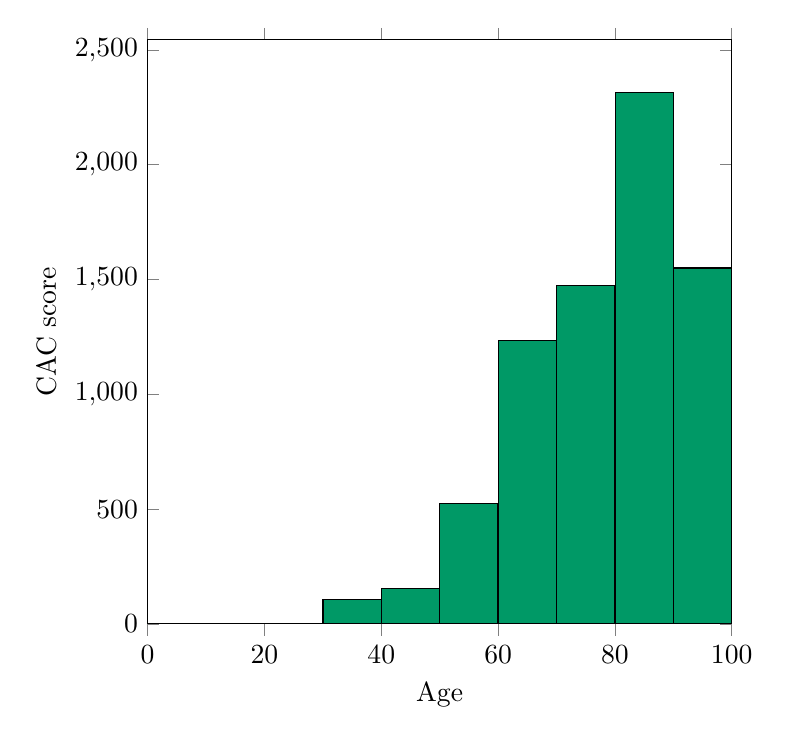
\begin{tikzpicture}
    \begin{axis}[
        name=cac_avg_by_age,height=9cm,width=9cm,
        ybar,
        ymin=0,ylabel={CAC score},
        xmin=0,xmax=100,xlabel={Age},
        bar width=21pt,
    ]
        \addplot[fill=green!60!blue] coordinates {
            (5,0)
            (15,0)
            (25,0)
            (35,107)
            (45,155)
            (55,525)
            (65,1234)
            (75,1474)
            (85,2313)
            (95,1550)
        };
    \end{axis}
\end{tikzpicture}
 }
		\end{subfigure}
	\end{figure}
\end{frame}


\begin{frame}{Dataset}
	\begin{figure}
		\centering
		\begin{subfigure}[b]{0.45\textwidth}
			\resizebox{\textwidth}{\textwidth}{ \begin{tikzpicture}
    \begin{axis}[
        name=cac_plot,at={($(age_plot.east)+(2cm,0)$)},anchor=west,height=9cm,width=9cm,
        % title={CAC score distribution},
        ybar,
        symbolic x coords={0, 1-10, 11-100, 101-400, >400},
        ymin=0,ylabel={Patients},
        xmin=0,xtick=data,xlabel={CAC score},
        bar width=30pt,
        enlarge x limits=0.1,
        % nodes near coords={\pgfmathprintnumber\pgfplotspointmeta} % put value on bar top
    ]
        \addplot[fill=orange!70] coordinates {
            (0,235)
            (1-10,10)
            (11-100,55)
            (101-400,64)
            (>400,239)
        };
    \end{axis}
\end{tikzpicture}
 }
		\end{subfigure}
		\begin{subfigure}[b]{0.45\textwidth}
			\resizebox{\textwidth}{\textwidth}{ 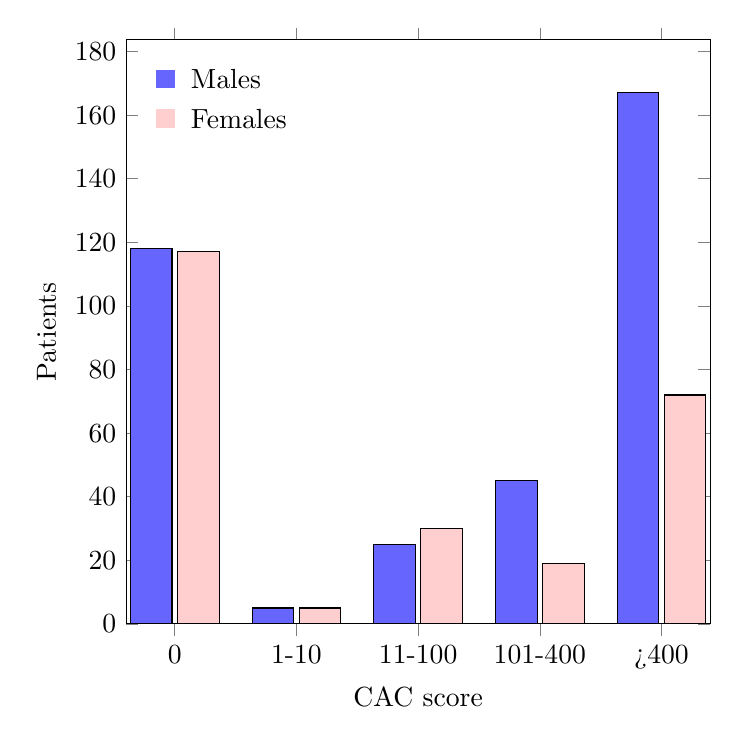
\begin{tikzpicture}
    \begin{axis}[
        name=cac_by_gender,height=9cm,width=9cm,
        % title={CAC score by gender distribution},
        ybar,
        symbolic x coords={0, 1-10, 11-100, 101-400, >400},
        ymin=0,ylabel={Patients},
        xmin=0,xtick=data,xlabel={CAC score},
        bar width=15pt,
        enlarge x limits=0.1,
        % nodes near coords={\pgfmathprintnumber\pgfplotspointmeta} % put value on bar top
    ]
        \addplot[fill=blue!60] coordinates {
            (0,118)
            (1-10,5)
            (11-100,25)
            (101-400,45)
            (>400,167)
        };
        \addplot[fill=pink!75] coordinates {
            (0,117)
            (1-10,5)
            (11-100,30)
            (101-400,19)
            (>400,72)
        };
    \end{axis}
    \node[fill=blue!60,xshift=0.5cm,yshift=-0.5cm] at (cac_by_gender.north west) (male) {};
    \node[right of=male,anchor=west,xshift=-0.8cm] {Males};
    \node[fill=pink!75,below of=male,yshift=0.5cm] (female) {};
    \node[right of=female,anchor=west,xshift=-0.8cm] {Females};
\end{tikzpicture}
 }
		\end{subfigure}\hspace{1em}
	\end{figure}
\end{frame}


\section{Experiments}\subsection{Experiments}


\begin{frame}{Detecting calcium from CT}
	\framesubtitle{Training teachers}
	\begin{columns}[onlytextwidth]
		\column{.1\linewidth}
			\begin{figure}
				\resizebox{\textwidth}{!}{ \includegraphics{heart_segmentation_axial} }
			\end{figure}			
		\column{.9\linewidth}
			\begin{itemize}
				\item 2D Cardiac area extraction on each CT slice using FPN pre-trained on ImageNet
			\end{itemize}
	\end{columns}
	\begin{columns}[onlytextwidth]
		\column{.7\linewidth}
			\begin{itemize}
				\item Training SimpleCT: 4-layers 3D CNN
				\item Training RetinaCT: ResNet extracted from RetinaNet pre-trained on LUNA16
			\end{itemize}
		\column{.27\linewidth}
			\begin{figure}
				\vspace{-3em}
				\resizebox{\textwidth}{!}{ \includegraphics{simple_ct_architecture} }
			\end{figure}
	\end{columns}
	\centering
	\begin{tabular}{|c<{\hspace{-1em}}l|c|c|c|c|}
		\hline
		\multicolumn{2}{|c|}{\textbf{Experiment}} & \textbf{Acc.} & \textbf{BA} & \textbf{Sens.} & \textbf{Spec.} \\
		\hline
		(T1) & SimpleCT 3-layer class.+l2-reg.       & 0.90          & 0.88          & \textbf{1.00} & 0.75 \\
		\hline
		(T2) & SimpleCT 1-layer class.               & 0.90          & \textbf{0.91} & 0.90          & \textbf{0.91} \\
		\hline
		(T3) & RetinaCT 3-layer class.+freeze+l2-reg & \textbf{0.92} & \textbf{0.91} & \textbf{1.00} & 0.81 \\
		\hline
	\end{tabular}
\end{frame}


\begin{frame}[t]{Detecting calcium from CXR}
	\framesubtitle{Reference results}
	\begin{columns}
		\column{\dimexpr\paperwidth-10pt}
		\centering
		\begin{tabular}{|c<{\hspace{-1em}}p{16em}|c|c|c|c|c|}
			\hline
			\multicolumn{2}{|c|}{\textbf{Experiment}}                     & \textbf{Teacher}        & \textbf{Acc.} & \textbf{BA}   & \textbf{Sens.}& \textbf{Spec.} \\
			\hhline{=======}
			(T1) & SimpleCT 3-layer class.+l2-reg.                        & N/A \cellcolor{gray!25} & 0.90          & 0.88          & \textbf{1.00} & 0.75 \\
			\hline
			(T2) & SimpleCT 1-layer class.                                & N/A \cellcolor{gray!25} & 0.90          & \textbf{0.91} & 0.90          & \textbf{0.91} \\
			\hline
			(T3) & RetinaCT 3-layer class.+freeze+l2-reg                  & N/A \cellcolor{gray!25} & \textbf{0.92} & \textbf{0.91} & \textbf{1.00} & 0.81 \\
			\hhline{=======}
			(A)  & SimpleCXR from scratch                                 & N/A \cellcolor{gray!25} & 0.67          & 0.61          & 0.84          & 0.38          \\
			\hline
			(B)  & DenseNet \citeauthor{iodice_2022},2022                 & N/A \cellcolor{gray!25} & \textbf{0.78} & \textbf{0.72} & \textbf{0.92} & \textbf{0.52} \\
			\hline
		\end{tabular}
	\end{columns}
	\vskip0pt plus.5fill
	\begin{columns}[onlytextwidth]
		\column{.7\linewidth}
			\begin{itemize}
				\item SimpleCXR: a 4-layers CNN, 2D version of SimpleCT
			\end{itemize}
		\column{.27\linewidth}
			\begin{figure}
				\resizebox{\textwidth}{!}{ \includegraphics{simple_cxr_architecture} }
			\end{figure}
	\end{columns}
\end{frame}


\begin{frame}[t]{Detecting calcium from CXR}
	\framesubtitle{Response-based knowledge distillation}
	\begin{columns}
		\column{\dimexpr\paperwidth-10pt}
		\centering
		\begin{tabular}{|c<{\hspace{-1em}}p{16em}|c|c|c|c|c|}
			\hline
			\multicolumn{2}{|c|}{\textbf{Experiment}}                     & \textbf{Teacher}        & \textbf{Acc.} & \textbf{BA}   & \textbf{Sens.}& \textbf{Spec.} \\
			\hhline{=======}
			(T1) & SimpleCT 3-layer class.+l2-reg.                        & N/A \cellcolor{gray!25} & 0.90          & 0.88          & \textbf{1.00} & 0.75 \\
			\hline
			(T2) & SimpleCT 1-layer class.                                & N/A \cellcolor{gray!25} & 0.90          & \textbf{0.91} & 0.90          & \textbf{0.91} \\
			\hline
			(T3) & RetinaCT 3-layer class.+freeze+l2-reg                  & N/A \cellcolor{gray!25} & \textbf{0.92} & \textbf{0.91} & \textbf{1.00} & 0.81 \\
			\hhline{=======}
			(A)  & SimpleCXR from scratch                                 & N/A \cellcolor{gray!25} & 0.67          & 0.61          & 0.84          & 0.38          \\
			\hline
			(B)  & DenseNet \citeauthor{iodice_2022},2022                 & N/A \cellcolor{gray!25} & \textbf{0.78} & \textbf{0.72} & \textbf{0.92} & \textbf{0.52} \\
			\hhline{=======}
			(1)  & SimpleCXR Resp-KD $\alpha\!\!=\!\!0.1$,$T\!\!=\!\!1$   & (T2)                    &         0.64  & 0.63          &         0.69  & \textbf{0.56} \\
			\hline
			(2)  & SimpleCXR Resp-KD $\alpha\!\!=\!\!0.5$,$T\!\!=\!\!1$   & (T3)                    & \textbf{0.72} & \textbf{0.64} & \textbf{0.93} &         0.35  \\
			\hline
		\end{tabular}
	\end{columns}
\end{frame}


\begin{frame}[t]{Detecting calcium from CXR}
	\framesubtitle{Feature-based knowledge distillation}
	\begin{columns}
		\column{\dimexpr\paperwidth-10pt}
		\centering
		\begin{tabular}{|c<{\hspace{-1em}}p{16em}|c|c|c|c|c|}
			\hline
			\multicolumn{2}{|c|}{\textbf{Experiment}}                     & \textbf{Teacher}        & \textbf{Acc.} & \textbf{BA}   & \textbf{Sens.}& \textbf{Spec.} \\
			\hhline{=======}
			(T1) & SimpleCT 3-layer class.+l2-reg.                        & N/A \cellcolor{gray!25} & 0.90          & 0.88          & \textbf{1.00} & 0.75 \\
			\hline
			(T2) & SimpleCT 1-layer class.                                & N/A \cellcolor{gray!25} & 0.90          & \textbf{0.91} & 0.90          & \textbf{0.91} \\
			\hline
			(T3) & RetinaCT 3-layer class.+freeze+l2-reg                  & N/A \cellcolor{gray!25} & \textbf{0.92} & \textbf{0.91} & \textbf{1.00} & 0.81 \\
			\hhline{=======}
			(A)  & SimpleCXR from scratch                                 & N/A \cellcolor{gray!25} & 0.67          & 0.61          & 0.84          & 0.38          \\
			\hline
			(B)  & DenseNet \citeauthor{iodice_2022},2022                 & N/A \cellcolor{gray!25} & \textbf{0.78} & \textbf{0.72} & \textbf{0.92} & \textbf{0.52} \\
			\hhline{=======}
			(1)  & SimpleCXR Resp-KD $\alpha\!\!=\!\!0.1$,$T\!\!=\!\!1$   & (T2)                    &         0.64  & 0.63          &         0.69  & \textbf{0.56} \\
			\hline
			(2)  & SimpleCXR Resp-KD $\alpha\!\!=\!\!0.5$,$T\!\!=\!\!1$   & (T3)                    & \textbf{0.72} & \textbf{0.64} & \textbf{0.93} &         0.35  \\
			\hhline{=======}
			(3)  & SimpleCXR Feat-KD encoder $\alpha\!\!=\!\!0.5$         & (T2)                    &         0.61  &         0.62  &         0.59  & \textbf{0.65} \\
			\hline
			(4)  & SimpleCXR Feat-KD branch $\alpha\!\!=\!\!0.5$          & (T1)                    & \textbf{0.69} & \textbf{0.64}  & \textbf{0.85} &         0.42  \\
			\hline
		\end{tabular}
	\end{columns}
\end{frame}


\begin{frame}[t]{Detecting calcium from CXR}
	\framesubtitle{Response-based knowledge distillation + transfer learning}
	\begin{columns}
		\column{\dimexpr\paperwidth-10pt}
		\centering
		\begin{tabular}{|c<{\hspace{-1em}}p{16em}|c|c|c|c|c|}
			\hline
			\multicolumn{2}{|c|}{\textbf{Experiment}}                     & \textbf{Teacher}        & \textbf{Acc.} & \textbf{BA}   & \textbf{Sens.}& \textbf{Spec.} \\
			\hhline{=======}
			(T1) & SimpleCT 3-layer class.+l2-reg.                        & N/A \cellcolor{gray!25} & 0.90          & 0.88          & \textbf{1.00} & 0.75 \\
			\hline
			(T2) & SimpleCT 1-layer class.                                & N/A \cellcolor{gray!25} & 0.90          & \textbf{0.91} & 0.90          & \textbf{0.91} \\
			\hline
			(T3) & RetinaCT 3-layer class.+freeze+l2-reg                  & N/A \cellcolor{gray!25} & \textbf{0.92} & \textbf{0.91} & \textbf{1.00} & 0.81 \\
			\hhline{=======}
			(A)  & SimpleCXR from scratch                                 & N/A \cellcolor{gray!25} & 0.67          & 0.61          & 0.84          & 0.38          \\
			\hline
			(B)  & DenseNet \citeauthor{iodice_2022},2022                 & N/A \cellcolor{gray!25} & \textbf{0.78} & \textbf{0.72} & \textbf{0.92} & \textbf{0.52} \\
			\hhline{=======}
			(1)  & SimpleCXR Resp-KD $\alpha\!\!=\!\!0.1$,$T\!\!=\!\!1$   & (T2)                    &         0.64  & 0.63          &         0.69  & \textbf{0.56} \\
			\hline
			(2)  & SimpleCXR Resp-KD $\alpha\!\!=\!\!0.5$,$T\!\!=\!\!1$   & (T3)                    & \textbf{0.72} & \textbf{0.64} & \textbf{0.93} &         0.35  \\
			\hhline{=======}
			(3)  & SimpleCXR Feat-KD encoder $\alpha\!\!=\!\!0.5$         & (T2)                    &         0.61  &         0.62  &         0.59  & \textbf{0.65} \\
			\hline
			(4)  & SimpleCXR Feat-KD branch $\alpha\!\!=\!\!0.5$          & (T1)                    & \textbf{0.69} & \textbf{0.64}  & \textbf{0.85} &         0.42  \\
			\hhline{=======}
			(5)  & DenseNet Resp-KD+TL $\alpha\!\!=\!\!0.5$,$T\!\!=\!\!1$ & (T1)                    & \textbf{0.77} &         0.70  & \textbf{0.94} &         0.46  \\
			\hline
			(6)  & DenseNet Resp-KD+TL $\alpha\!\!=\!\!0.1$,$T\!\!=\!\!1$ & (T3)                    & 0.76          & \textbf{0.71} &         0.88  & \textbf{0.54} \\
			\hline
		\end{tabular}
	\end{columns}
\end{frame}


\section{Conclusion}\subsection{Conclusion}


\begin{frame}{Conclusion}
	\begin{itemize}
		\item KD is an emerging technique and find the proper strategy and model architecture is still an open point
		\item KD can be a tool at disposal, maybe mixed with other techniques, to mitigate impact of limited amount of data
	\end{itemize}

	Possible improvements:
	\begin{itemize}
		\item Collect more samples in the intermediate risk classes could help response-based KD to find hidden relationships between them
		\item Dataset is biased towards positive class: a balanced loss could improve specificity
		\item SimpleCXR could be too simple: explore other architectures
	\end{itemize}
\end{frame}


\appendix
\section*{Appendix}\subsection*{Appendix}
\ClearShipoutPictureFG


\begin{frame}[plain,noframenumbering]
	\begin{center}
		\usebeamercolor[fg]{titlegraphic}\inserttitlegraphic\par
		\usebeamerfont{title}\textbf{Grazie}\par
	\end{center}
\end{frame}

\SetLogo

\begin{frame}[noframenumbering]{Dataset}
	\centering
	\resizebox{0.6\textwidth}{!}{
		\begin{tabular}{|l|r c|r c|c|}
			\hline
			& \multicolumn{2}{c|}{\textbf{Negatives}} & \multicolumn{2}{c|}{\textbf{Positives}} & \textbf{TOTAL} \\
			\hline
			Male    & 118 & (32,8\%) & 242 & (67,2\%) & 360 \\
			Female  & 117 & (48,1\%) & 126 & (51,9\%) & 243 \\
			\hline
			Age 0-9   &   1 &  (100\%) &   0 &    (0\%) &   1 \\
			Age 10-19 &  13 &  (100\%) &   0 &    (0\%) &  13 \\
			Age 20-29 &  28 &  (100\%) &   0 &    (0\%) &  28 \\
			Age 30-39 &  28 & (96,6\%) &   1 &  (3,4\%) &  29 \\
			Age 40-49 &  47 & (79,7\%) &  12 & (20,3\%) &  59 \\
			Age 50-59 &  54 & (52,9\%) &  48 & (47,1\%) & 102 \\
			Age 60-69 &  42 & (29,0\%) & 103 & (71,0\%) & 145 \\
			Age 70-79 &  13 &  (9,8\%) & 120 & (90,2\%) & 133 \\
			Age 80-89 &   8 & (10,0\%) &  72 & (90,0\%) &  80 \\
			Age 90+   &   1 &  (7,7\%) &  12 & (92,3\%) &  13 \\
			\hline
			\hline
			Training set   & 164 & (40.3\%) & 243 & (59.7\%) &    407 \\
			Test set (CT)  &  32 & (38.1\%) &  52 & (61.9\%) &     84 \\
			Test set (CXR) &  71 & (36.2\%) & 125 & (63.8\%) & 84+112 \\
			\hline
			\hline
			ALL       & 235 & (39,0\%) & 368 & (61,0\%) & 603 \\
			\hline
		\end{tabular}
	}
\end{frame}


\end{document}